\subsection[Classificatori Naïve Bayes]{\textit{Classificatori Naïve Bayes}}
%\subsubsection[Osservazioni per la regressione]{Osservazioni per la regressione}


\begin{frame}
	
	\frametitle{Classificatori Naïve Bayes}
	\begin{columns}
	
		\column{0.5\linewidth}
		\begin{figure}[!htbp]
			\centering
			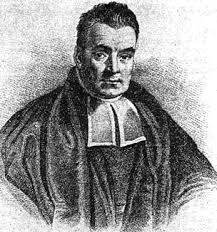
\includegraphics[width=0.93\linewidth]{images/supervised/naive_bayes/thomas_bayes_1.jpg}
%			\caption{}
%			\label{} 
		\end{figure}
		
		
		
		\column{0.5\linewidth}
		\begin{figure}[!htbp]
			\centering
			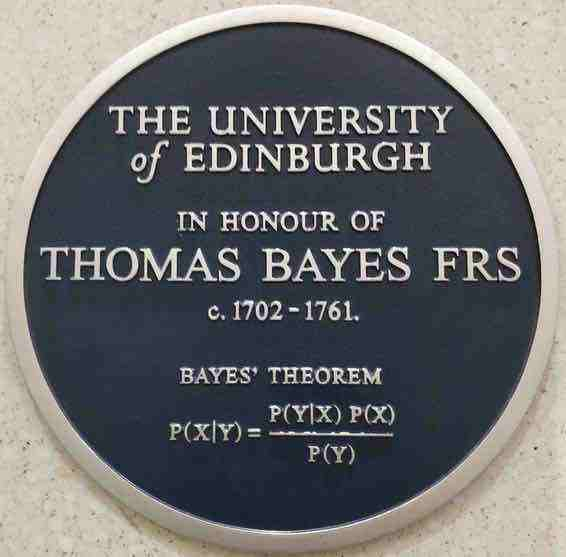
\includegraphics[width=1.0\linewidth]{images/supervised/naive_bayes/thomas_bayes_2.jpg}
%			\caption{}
%			\label{} 
		\end{figure}
		
	\end{columns}
	
	
\end{frame}

\begin{frame}
	
	\frametitle{Classificatori Naïve Bayes}
		I metodi naif Bayes sono un insieme di algoritmi di apprendimento supervisionato \textbf{basati sull'applicazione del teorema di Bayes} con l'assunzione ``naïf'' dell'indipendenza condizionale tra ogni coppia di features dato il valore della variabile di classe (label).
		\pause
		\newlinedouble
		Il classificatore bayesiano naif, o \textbf{Naïve Bayes}, presenta una somiglianza maggiore con i percettroni rispetto all’albero di decisione, perché è basato su un insieme di valori raggruppati per ottenere una previsione.
		\pause
		\newlinedouble
		Anche il classificatore bayesiano naif, come il percettrone e l’albero di decisione, è un algoritmo storico \textbf{utilizzato fin dagli anni Cinquanta}, sebbene con un nome diverso e forme leggermente differenti.
	
\end{frame}


\begin{frame}
	
	\frametitle{Concetti di base di probabilità}
%	\begin{block}{Concetti di base di probabilità}
	
		\begin{itemize}
			\item Spazio degli eventi ($\Omega$): dominio di una variabile casuale $X$
			\item Misura di probabilità $P(\bullet)$
				\begin{itemize}
					\item[--] $P$ è una misura su $\Omega$
					\item[--] $P(X = x \in \Omega)$ è una misura della fiducia in $X = x$
				\end{itemize}
			\item Assiomi di Kolmogorov:
				\begin{enumerate}
					\item La probabilità di un evento è un numero reale non negativo:\\
						$\forall x \in \Omega, \quad 0 \leq P(X = x) \leq 1$
					\item La probabilità dell'intero spazio campione è 1:\\
						$P(\Omega) = 1$
					\item Qualsiasi sequenza numerabile di insiemi disgiunti  $X_1, X_2, \dots$ soddisfa:\\
						$\forall X_1, X_2,\dots \ni i \neq j \rightarrow X_i \land X_j = \varnothing$\\
						$P \left( \cup_{i=1}^{\infty} X_i \right) = \sum_{i=1}^{\infty} P(X_i)$
				\end{enumerate}
			\item Probabilità congiunta: $P(X_1 \land X_2) \equiv$ dell’evento $X_1 \land X_2$
			\item Indipendenza: $P(X_1 \land X_2) = P(X_1)P(X_2)$
		\end{itemize}
%	\end{block}
	
\end{frame}


\begin{frame}
	
	\frametitle{Teorema di Bayes}
%	\begin{block}{Teorema di Bayes}
			Considerando un insieme di alternative $X_1,\ldots,X_n$ che partizionano lo spazio degli eventi $\Omega$ (ossia $\ X_i\cap X_j=\varnothing\ \forall i \neq j$ e $\cup_{i=1}^n X_i=\Omega$) si trova la seguente espressione per la probabilità condizionata:
				\begin{empheq}[box=\fcolorbox{blue!40!black!60}{yellow!10}]{align*}
					P(X_i \vert E) = \frac{P(E \vert X_i) P(X_i)}{P(E)}
				\end{empheq}
				%$$P(X_i|E) = \frac{P(E | X_i) P(X_i)}{P(E)}$$% = \frac{P(E | X_i) P(X_i)}{\sum_{j=1}^n P(E | X_j) P(X_j)}$$

		Dove:
		\begin{itemize}
			\item $P(X_i)$ è la probabilità a priori o probabilità marginale di $X_i$. \textit{A priori} significa che non tiene conto di nessuna informazione riguardo $E$
			\item $P(X_i \vert E)$ è la probabilità condizionata di $X_i$, noto $E$. Viene anche chiamata probabilità a posteriori, visto che è derivata o dipende dallo specifico valore di $E$.
			\item $P(E \vert X_i)$ è la probabilità condizionata di $E$, noto $X_i$
			\item $P(E)$ è la probabilità a priori di $E$, e funge da costante di normalizzazione
		
		\end{itemize}

%	\end{block}
	
\end{frame}


\begin{frame}
	
	\frametitle{Teorema di Bayes}
		
	\begin{figure}[!htbp]
		\centering
		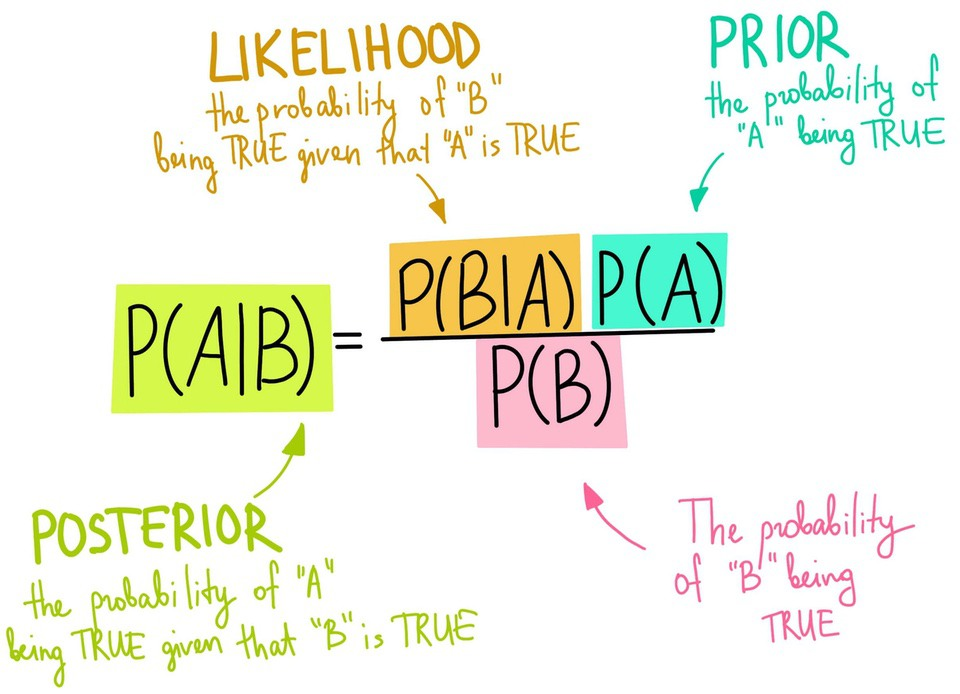
\includegraphics[width=0.8\linewidth]{images/supervised/naive_bayes/bayes_rule.jpeg}
%		\caption{}
	\end{figure}
	
\end{frame}


\begin{frame}
	
	\frametitle{Classificatori Naïve Bayes: l'algoritmo parte 1}
	
	In termini di classificazione il teorema di Bayes afferma che, data la variabile di classe $y$ (label) e il vettore delle features da $x_1$ a $x_n$, la seguente relazione è vera:
	$$P(y \vert x_1, \dots, x_n) = \frac{P(y) P(x_1, \dots, x_n \vert y)}
                                 {P(x_1, \dots, x_n)}$$
                              
	Poiché si assume in maniera naif che le features siano indipendenti tra loro:
	$$P(x_1, \dots, x_n \vert y) = \prod_{i=1}^{n} P(x_i \vert y)$$
	
	si può semplificare questa relazione in:
	$$P(y \vert x_1, \dots, x_n) = \frac{P(y) \prod_{i=1}^{n} P(x_i \vert y)}
                                 {P(x_1, \dots, x_n)}$$
\end{frame}


\begin{frame}
	
	\frametitle{Classificatori Naïve Bayes: l'algoritmo parte 2}

	Poiché $P(x_1, \dots, x_n)$ è costante al variare di $y$,\\ possiamo scrivere la seguente regola di classificazione:
	$$P(y \vert x_1, \dots, x_n) \propto P(y) \prod_{i=1}^{n} P(x_i \vert y) \quad \Rightarrow \quad \hat{y} = \arg\max_y P(y) \prod_{i=1}^{n} P(x_i \vert y)$$

	e possiamo usare la stima Maximum A Posteriori (MAP) per stimare:
	\begin{itemize}
		\item $P(y)$: ovvero la frequenza relativa della classe $y$ nel training set
		\item $P(x_i \vert y)$: i diversi classificatori Naïve Bayes differiscono principalmente per le ipotesi che fanno riguardo a questa distribuzione.
	\end{itemize}
	\ \\
	Nonostante le loro assunzioni apparentemente eccessivamente naif, i classificatori bayes naif hanno funzionato piuttosto bene in molte situazioni del mondo reale, notoriamente la classificazione dei documenti e il filtro dello spam.
\end{frame}


\begin{frame}
	
	\frametitle{Classificatori Naïve Bayes: l'algoritmo parte 3}
	
	A seconda delle ipotesi che si fanno riguardo alla distribuzione di $P(x_i \vert y)$ abbiamo:
	\begin{itemize}
		\item Gaussian Naïve Bayes%\\
			%Si presume che la likelihood delle features sia gaussiana:
			%$P(x_i \mid y) = \frac{1}{\sqrt{2\pi\sigma^2_y}} \exp\left(-\frac{(x_i - \mu_y)^2}{2\sigma^2_y}\right)$
		\item Multinomial Naïve Bayes%\\
			%$P(x_i \mid y) = \hat{\theta}_{yi} = \frac{ N_{yi} + \alpha}{N_y + \alpha n}$
		\item Complement Naïve Bayes
		\item Bernoulli Naïve Bayes
		\item Categorical Naïve Bayes
	\end{itemize}
	\ \\
	Ci focalizzeremo sul funzionamento del \textbf{Multinomial Naive Bayes} all'interno del quale le likelihood delle features sono approssimate con semplici frequenze relative.
	\newlinedouble
	Per approfondire gli altri modelli di Naïve Bayes leggere: \underline{\href{https://scikit-learn.org/stable/modules/naive_bayes.html}{scikit-learn Naive Bayes}}
\end{frame}



\begin{frame}
	
	\frametitle{Multinomial Naive Bayes}
	
	La distribuzione è parametrizzata dal vettore $\theta_y = (\theta_{y1},\ldots,\theta_{yn})$ per ogni classe $y$, dove $n$ è il numero di features e $\theta_{yi}$ è la probabilità $P(x_i \mid y)$ che la feature $i$ appaia in un campione appartenente alla classe $y$.
	\newlinedouble
	I parametri $\theta_y$ sono stimati da una versione smoothed della massima verosimiglianza, ovvero con la frequenza relativa:
	$$\hat{P(x_i \mid y)} = \hat{\theta}_{yi} = \frac{ N_{yi} + \alpha}{N_y + \alpha n}$$
	Dove:
	\begin{itemize}
		\item $N_{yi} = \sum_{x \in T} x_i$ è il numero di volte in cui la caratteristica $i$ appare in un campione di classe $y$ nel training set $T$
		\item $N_{y} = \sum_{i=1}^{n} N_{yi}$ è il conteggio totale di tutte le features per la classe $y$
		\item Per $\alpha = 1$ si applica uno smoothing di Laplace, mentre per $\alpha < 1$ si applica uno smoothing di Lidstone.\\
			Leggere più avanti per capirne lo scopo.
	\end{itemize}

\end{frame}


\begin{frame}
	
	\frametitle{Multinomial Naive Bayes: il problema della frequenza-zero}	
	
	Se non introducessimo il fattore $\alpha$, ovvero se calcolassimo $\theta_{yi}$ come segue:
	$$\hat{\theta}_{yi} = \frac{N_{yi}}{N_y}$$
	cosa succederebbe se il valore di un attributo non compare con un certo valore di classe $y$ (ovvero se $N_{yi} = 0$)?
	\pause
	\begin{itemize}
		\item La probabilità è zero! $\qquad \qquad \qquad \quad \text{ } \rightarrow P(x_i \vert y) = 0$
		\item La probabilità a posteriori diventa zero! $\rightarrow P(y \vert x_1, \dots, x_n) = 0$
	\end{itemize}
	\pause
	\ \\
	\textbf{Possibile rimedio}:\\
		per tener conto di eventi rari, si operano degli aggiustamenti sulle probabilita detti smoothing: ad esempio sommando 1 al conteggio di ogni combinazione attributo-classe. Il che corrisponde al caso $\alpha = 1$, ovvero applicare uno smoothing di Laplace.

\end{frame}


\begin{frame}
	
	\frametitle{Classificatori Naïve Bayes: l'algoritmo completo}
	
	%In conclusione, per restituire la classe di un esempio, l’algoritmo procede in questo modo:
	\begin{enumerate}
		\item apprende le probabilità che mettono in connessione le features-classi
			\begin{scriptsize}
			\begin{empheq}[box=\fcolorbox{blue!40!black!60}{yellow!10}]{align*}
				P(x_i \vert y) \quad \forall x_i \in X \text{ e } \forall y \in \mathbb{C}
			\end{empheq}	
			\end{scriptsize}
		\pause
		\item moltiplica tutte le probabilità correlate a ciascuna classe risultante, il tutto moltiplicato per la probabilità della specifica classe
			\begin{scriptsize}
			\begin{empheq}[box=\fcolorbox{blue!40!black!60}{yellow!10}]{align*}
				\Bbbk(y) = P(y) \prod_{i=1}^{n} P(x_i \vert y) \quad \forall y \in \mathbb{C}
			\end{empheq}
			\end{scriptsize}
		\pause
		\item normalizza le probabilità dividendo ognuna per la loro somma totale
			\begin{scriptsize}
			\begin{empheq}[box=\fcolorbox{blue!40!black!60}{yellow!10}]{align*}
				P(\dot{y} \vert x_1, x_2, \dots, x_n) = \frac{\Bbbk(\dot{y})}{\sum_{y=1}^{\mathbb{C}} \Bbbk(y)} \quad \rightarrow \quad  \text{ probabilità di appartenere alla classe } \dot{y}
			\end{empheq}
			\end{scriptsize}
		\pause
		\item prende come risposta la classe che mostra la più alta probabilità
			\begin{scriptsize}
			\begin{empheq}[box=\fcolorbox{blue!40!black!60}{yellow!10}]{align*}
				\hat{y} = \arg\max_y \Bbbk(y) = \arg\max_y P(y) \prod_{i=1}^{n} P(x_i \vert y) = \arg\max_y P(y \vert x_1, x_2, \dots, x_n)
			\end{empheq}
			\end{scriptsize}
	\end{enumerate}

\end{frame}


\begin{frame}
	
	\frametitle{Multinomial Naive Bayes:  un esempio parte 1}	
	
	Il problema consiste nel decidere se giocare a golf (oppure no) in base a determinate caratteristiche.\\
	Le caratteristiche sono quattro: overcast (meteo), temp (temperatura), humidity (umidità), windy (forza del vento).
	\begin{figure}[!htbp]
		\centering
		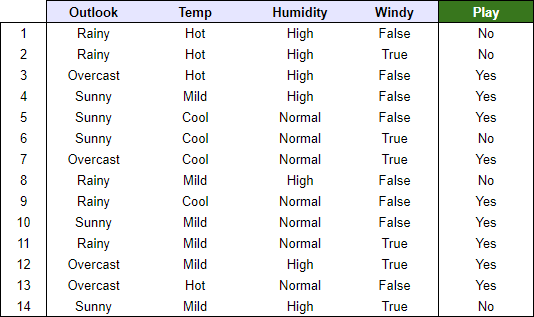
\includegraphics[width=0.7\linewidth]{images/supervised/naive_bayes/naive-bayes-esempio-1.png}
%			\caption{}
%			\label{} 
	\end{figure}
	

\end{frame}


\begin{frame}
	
	\frametitle{Multinomial Naive Bayes:  un esempio parte 2}	
	
	Per ogni caratteristica costruisco la tavola delle frequenze.
	\begin{figure}[!htbp]
		\centering
		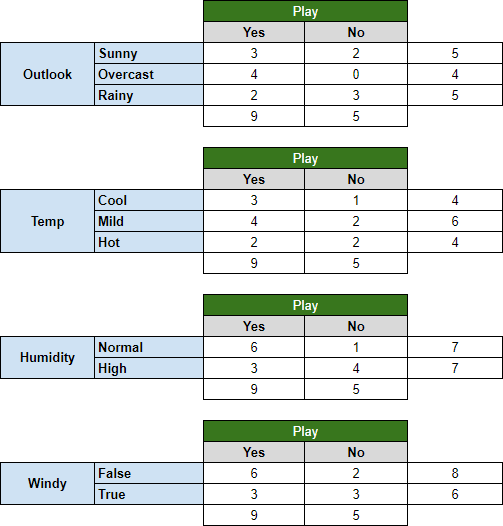
\includegraphics[width=0.5\linewidth]{images/supervised/naive_bayes/naive-bayes-esempio-2.png}
%			\caption{}
%			\label{} 
	\end{figure}
	

\end{frame}


\begin{frame}
	
	\frametitle{Multinomial Naive Bayes:  un esempio parte 3}
	
	Poi trasformo le frequenze in probabilità.
	
	\begin{figure}[!htbp]
		\centering
		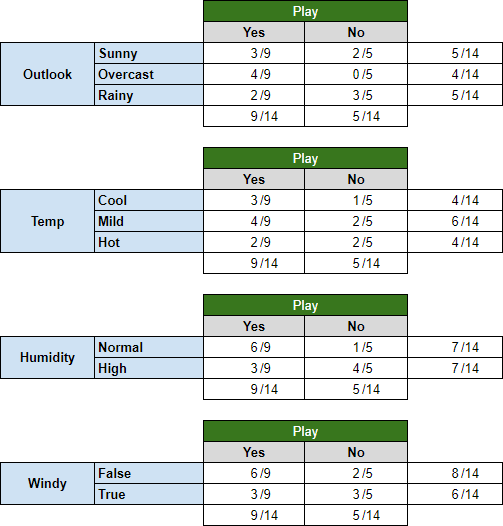
\includegraphics[width=0.5\linewidth]{images/supervised/naive_bayes/naive-bayes-esempio-3.png}
%			\caption{}
%			\label{} 
	\end{figure}
	

\end{frame}


\begin{frame}
	
	\frametitle{Multinomial Naive Bayes:  un esempio parte 4}	
	
	Ho tutte le informazioni utili per calcolare le probabilità semplici e le probabilità condizionate.
	
	\begin{figure}[!htbp]
		\centering
		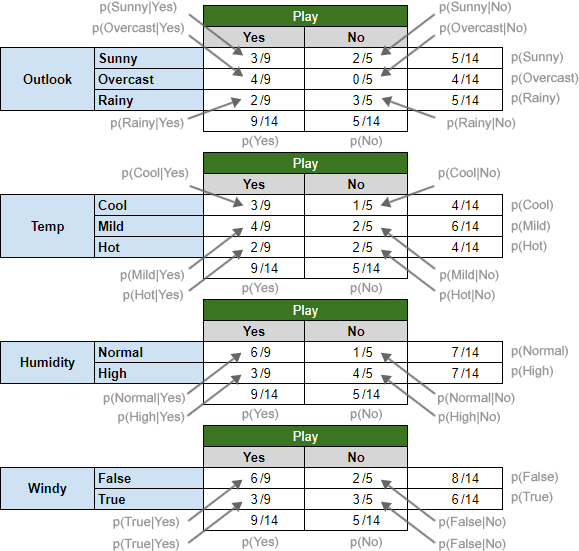
\includegraphics[width=0.5\linewidth]{images/supervised/naive_bayes/naive-bayes-esempio-4.png}
%			\caption{}
%			\label{} 
	\end{figure}
	

\end{frame}


\begin{frame}
	
	\frametitle{Multinomial Naive Bayes:  un esempio parte 5}	
	
	A questo punto il modello è pronto per essere utilizzato.\\
	Ad esempio, se le condizioni di ambiente $X$ sono le seguenti:
	\begin{itemize}
		\item Outlook=Rainy
		\item Temp=Cool
		\item Humidity=High
		\item Windy=True
	\end{itemize}
	\pause
	\ \\
	L'algoritmo calcola la probabilità della decisione di giocare, oppure no, moltiplicando tra loro le probabilità condizionali:
	$$\begin{cases} P(Yes|X)=P(Rainy|Yes) P(Cool|Yes) P(High|Yes) P(True|Yes) P(Yes) \\P(\text{ }No|X)=P(Rainy|No\text{ }) P(Cool|No\text{ }) P(High|No\text{ }) P(True|No\text{ }) P(No)
	\end{cases}$$
\end{frame}


\begin{frame}
	
	\frametitle{Multinomial Naive Bayes:  un esempio parte 6}	
		
	
	Sostituisco i valori delle probabilità condizionate:
	$$\begin{cases} P(Yes|X)=(2/9) (3/9) (3/9) (3/9) (9/14) \\ P(\text{ }No|X)=(3/5) (1/5) (4/5) (3/5) (5/14) \end{cases} \Rightarrow \begin{cases} P(Yes|X)=0.00529 \\ P(\text{ }No|X)=0.02057 \end{cases}$$

	Infine, normalizzo i risultati:
	$$\begin{cases} P(Yes|X)=\frac{0.00529}{0.00529+0.02057} \\ P(\text{ }No|X)=\frac{0.02057}{0.00529+0.02057} \end{cases} \Rightarrow \begin{cases} P(Yes|X)=0.20 \\ P(\text{ }No |X)=0.80 \end{cases}$$
	
	In conclusione, considerando le circostanze date dall'input $x_1, x_2, \dots, x_n$:
	\begin{itemize}
		\item $P(Yes \vert X) = 20\% \rightarrow$ la probabilità di giocare è del 20\%
		\item $P(\text{ }No \vert X) = 80\% \rightarrow$ la probabilità opposta di non giocare è del 80\%
	\end{itemize}
	
\end{frame}


\begin{frame}
	
	\frametitle{Classificatori Naïve Bayes: problematiche}
	
	Moltiplicare le probabilità va benissimo, però ci sono però alcune questioni da tenere presenti:
	\begin{itemize}
		\item risolvere i problemi di probabilità zero applicando la correzione di Laplace
		\item convertire le feature numeriche in variabili qualitative, perché la stima delle probabilità per le classi che comprendono range numerici è più facile
		%\item usare solo feature con valori pari o superiori a zero, anche se alcune varianti dell’algoritmo possono gestire anche le feature binarie e i valori negativi
		\item inserire valori nelle feature mancanti (in particolare quando nel calcolo andrebbe persa una probabilità importante) e contemporaneamente rimuovere quelle ridondanti e irrilevanti
		\item in particolare, le feature irrilevanti possono influire parecchio sui risultati. Una possibile soluzione consiste nel selezionare le feature, applicando un filtro in modo da considerare solamente le più importanti
	\end{itemize}
\end{frame}


\begin{frame}
	
	\frametitle{Classificatori Naïve Bayes: osservazioni}
	
	\begin{itemize}
		\item richiedono una piccola quantità di dati di addestramento per stimare i parametri necessari
		\item possono essere estremamente veloci rispetto a metodi più sofisticati
		\item l'assunzione di indipendenza condizionale significa che ogni distribuzione può essere stimata indipendentemente come una distribuzione unidimensionale (allevia curse of dimensionality)
		\item sebbene il Naïve Bayes sia noto come un buon classificatore, è noto per essere un cattivo stimatore, quindi gli output probabilistici non devono essere presi troppo sul serio
	\end{itemize}	
	
	\begin{figure}[!htbp]
		\centering
		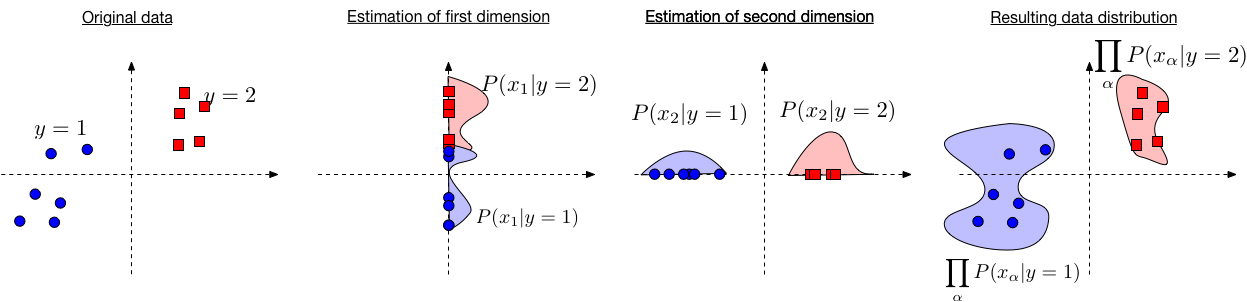
\includegraphics[width=0.95\linewidth]{images/supervised/naive_bayes/NBschematic.png}
%		\caption{}
	\end{figure}
%	
%	
\end{frame}